\section{Ход работы, результаты}
\subsection{Вид осциллограмм}
\begin{figure}[h]
    \centering
    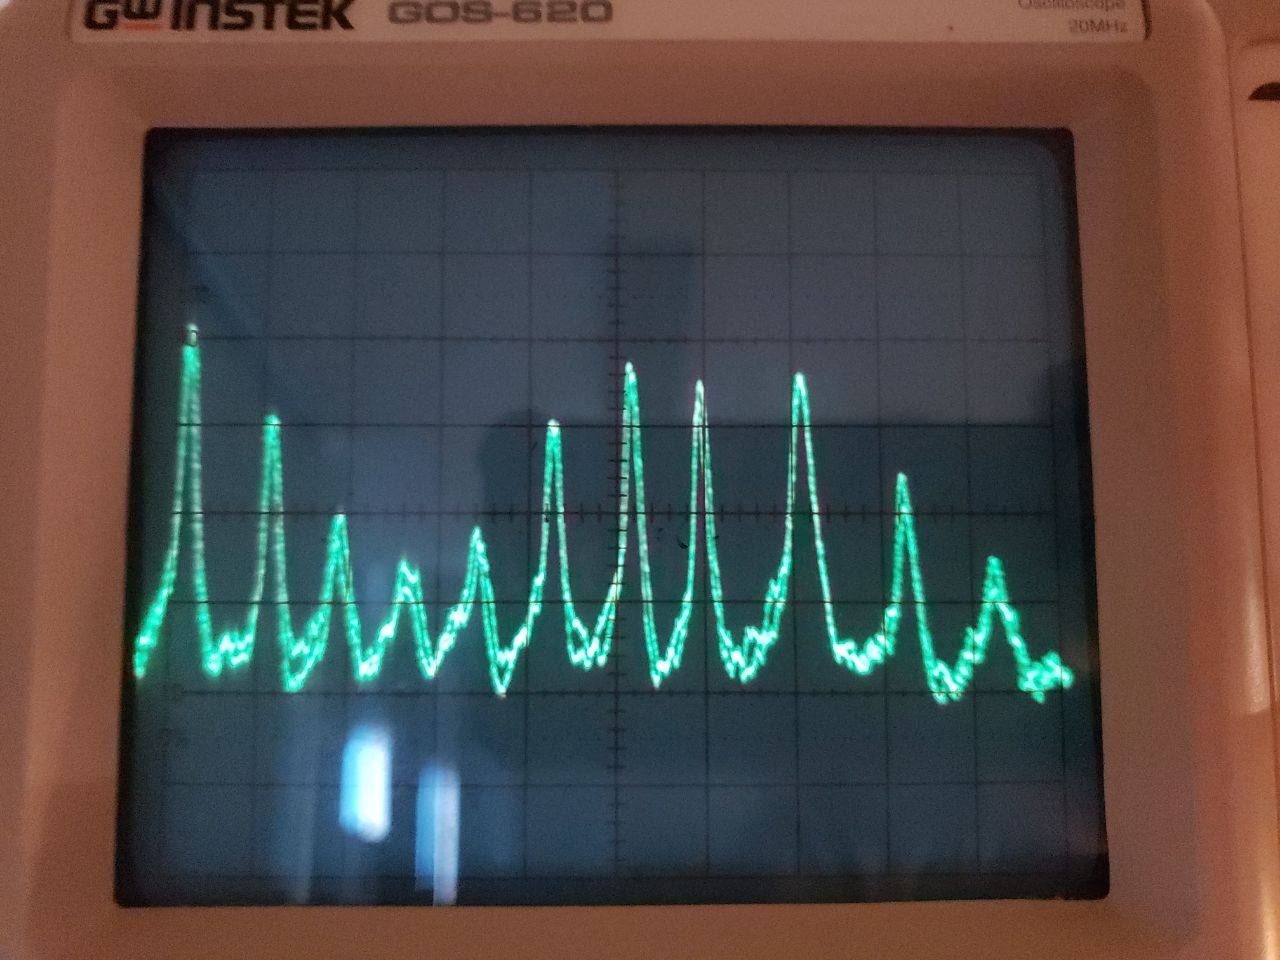
\includegraphics[width=0.4\textwidth]{oscar.jpg}
    \caption{Осциллограмма спектра лазерного излучения}
    \label{fig:oscar}
\end{figure}

После настройки приборов на осциллографе была получена картина спектра лазера, изображённая на рис. \ref{fig:oscar}. На ней полностью виден один доплеровский контур, а также половина ещё одного. При уменьшении напряжения на пьезокристалле амплитуда колебаний длины интерферометра и, следовательно, его спектра пропускания, количество мод, укладывающихся в получаемую картину, уменьшается. Это показано на рисунках \ref{fig:oscs}.
\newpage

\begin{figure}[h]
     \centering
     \begin{subfigure}[b]{0.3\textwidth}
         \centering
         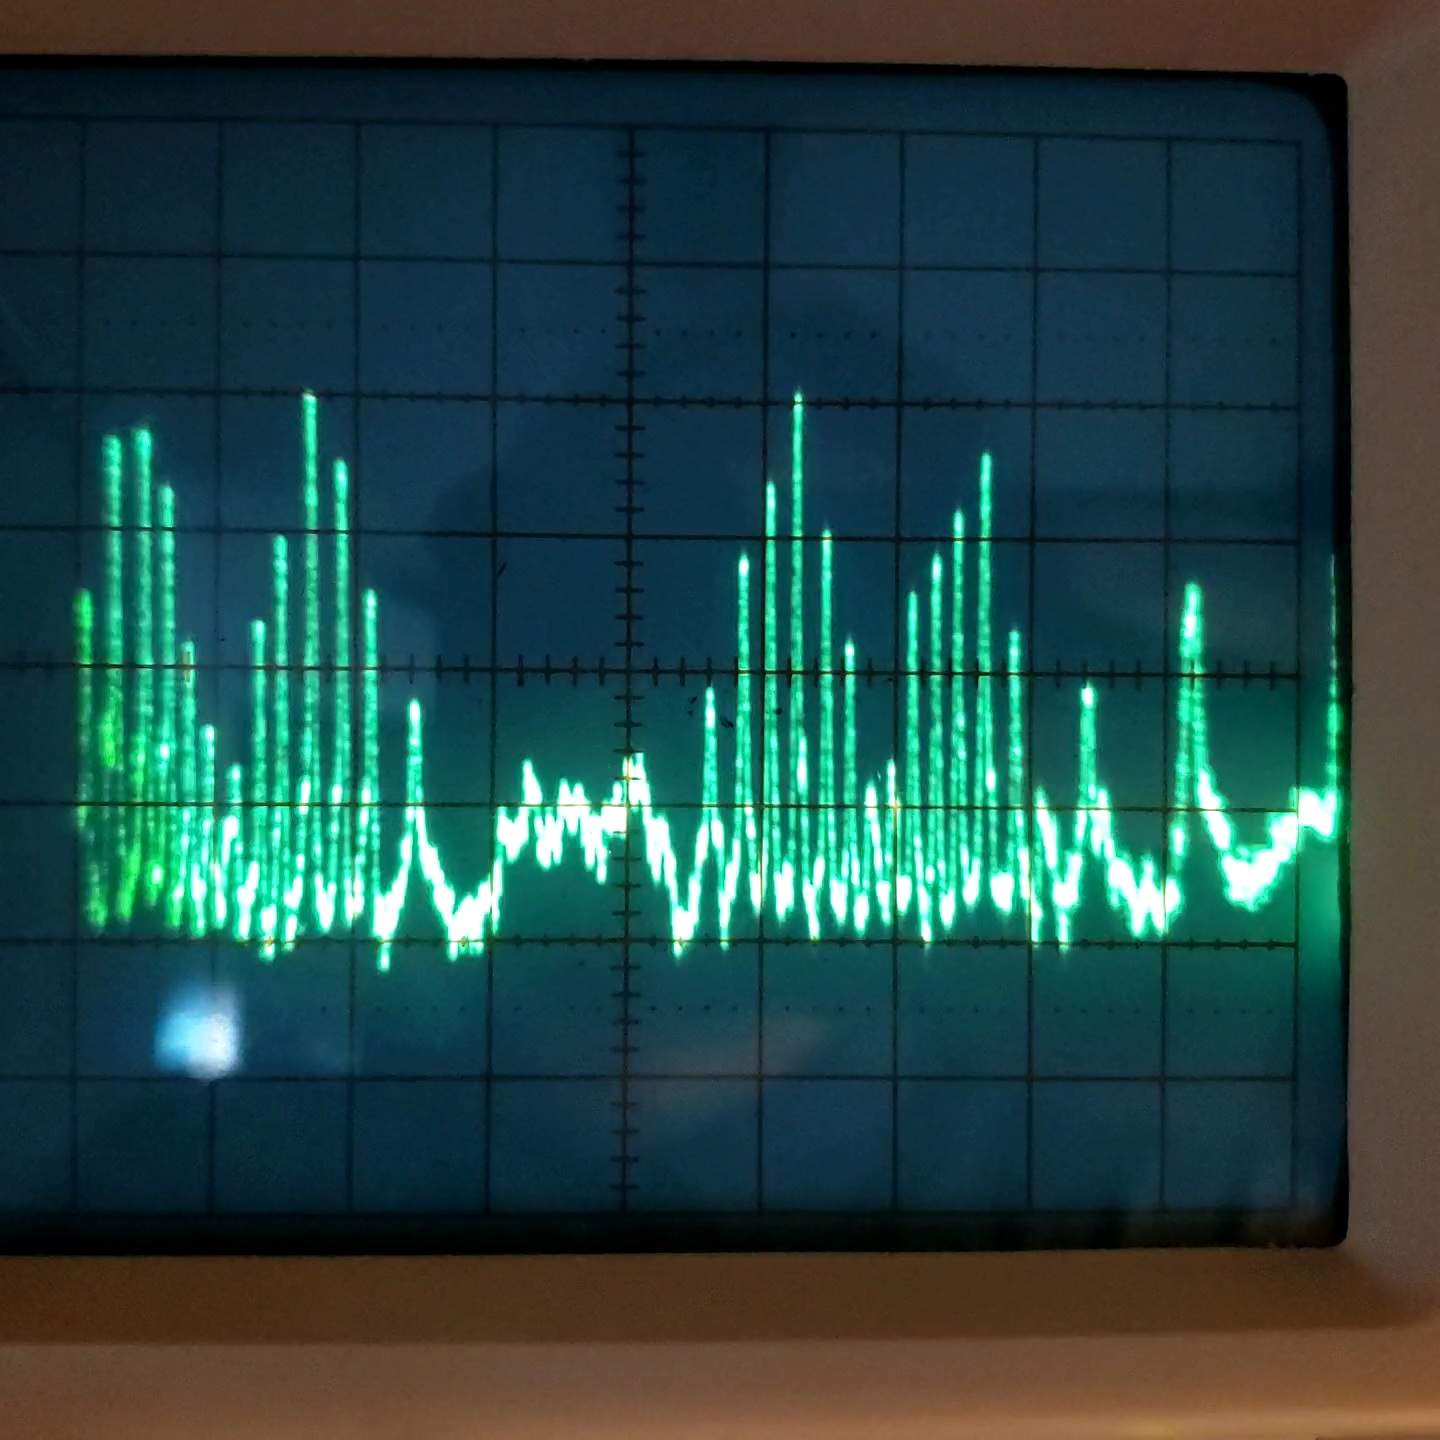
\includegraphics[width=\textwidth]{oscHigh.jpg}
         \caption{}
         \label{fig:high}
     \end{subfigure}
     \hfill
     \begin{subfigure}[b]{0.3\textwidth}
         \centering
         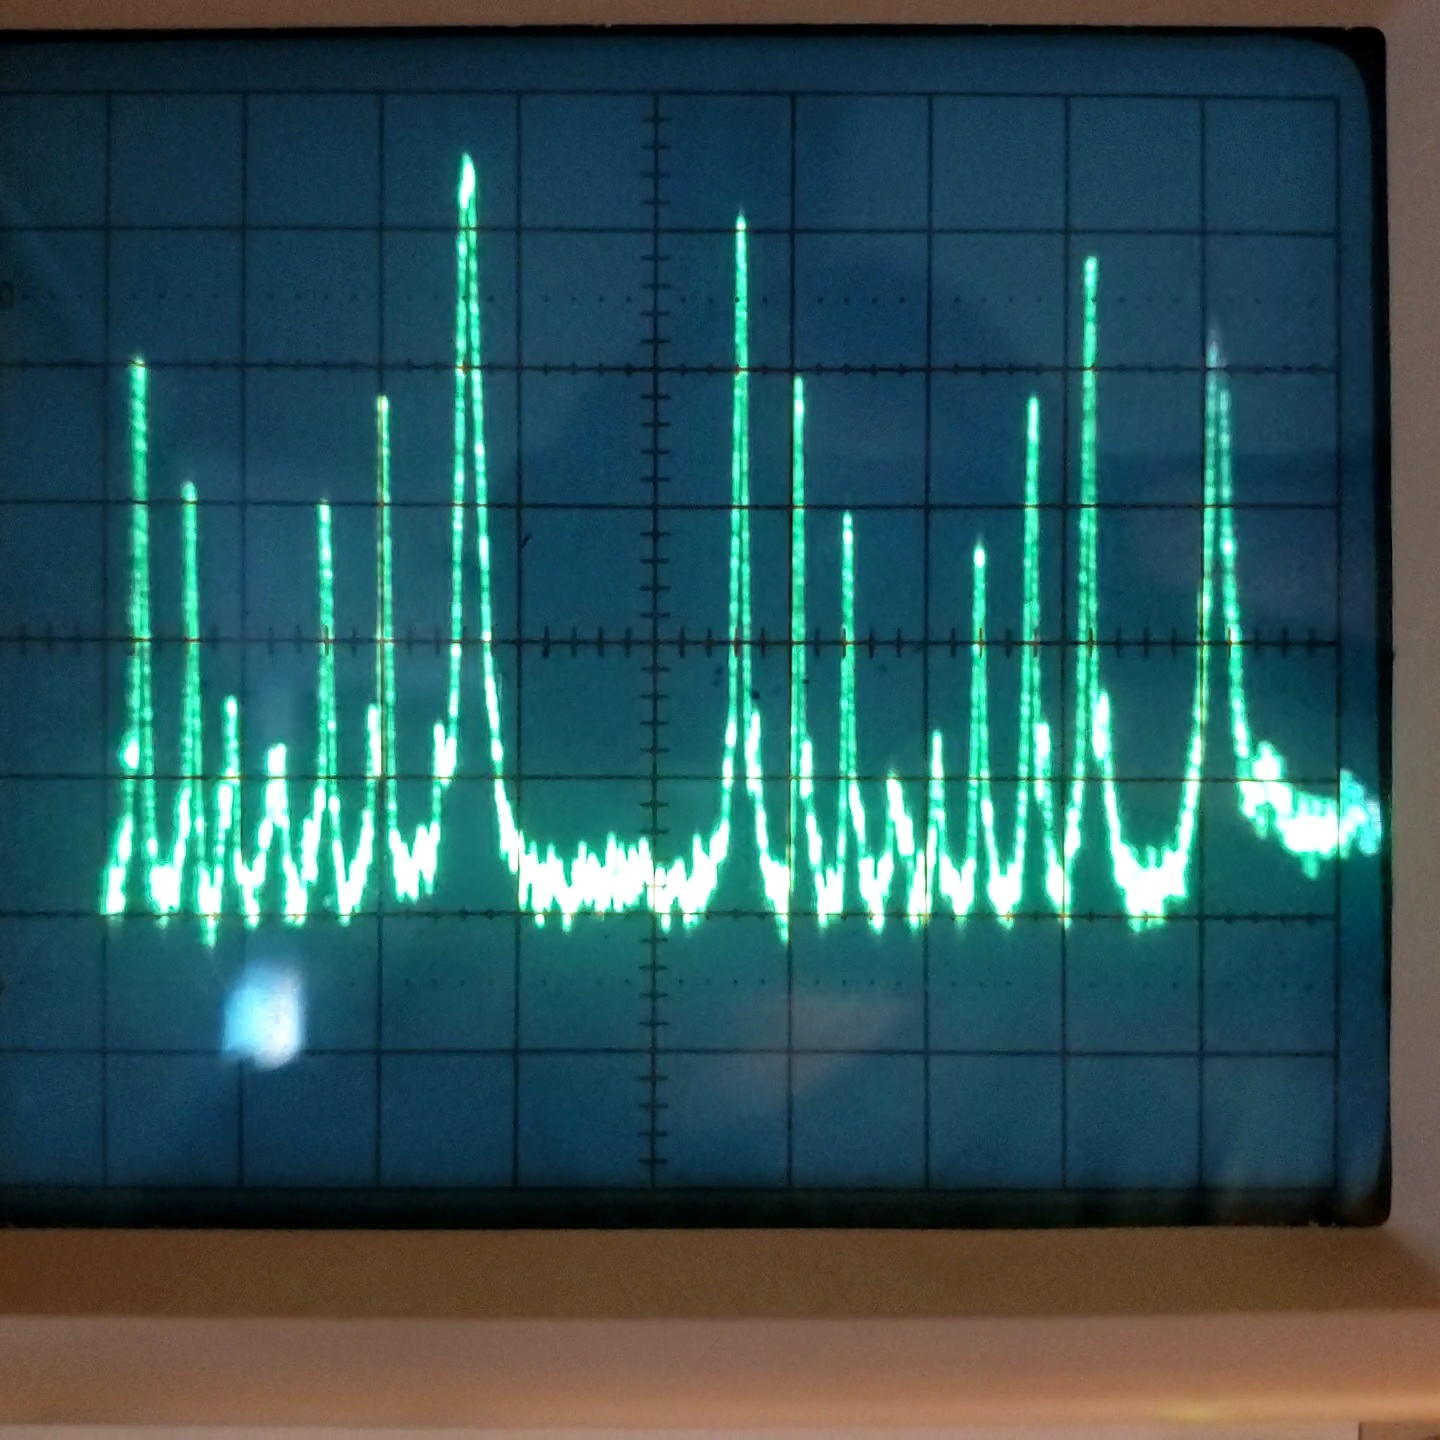
\includegraphics[width=\textwidth]{oscMed.jpg}
         \caption{}
         \label{fig:med}
     \end{subfigure}
     \hfill
     \begin{subfigure}[b]{0.3\textwidth}
         \centering
         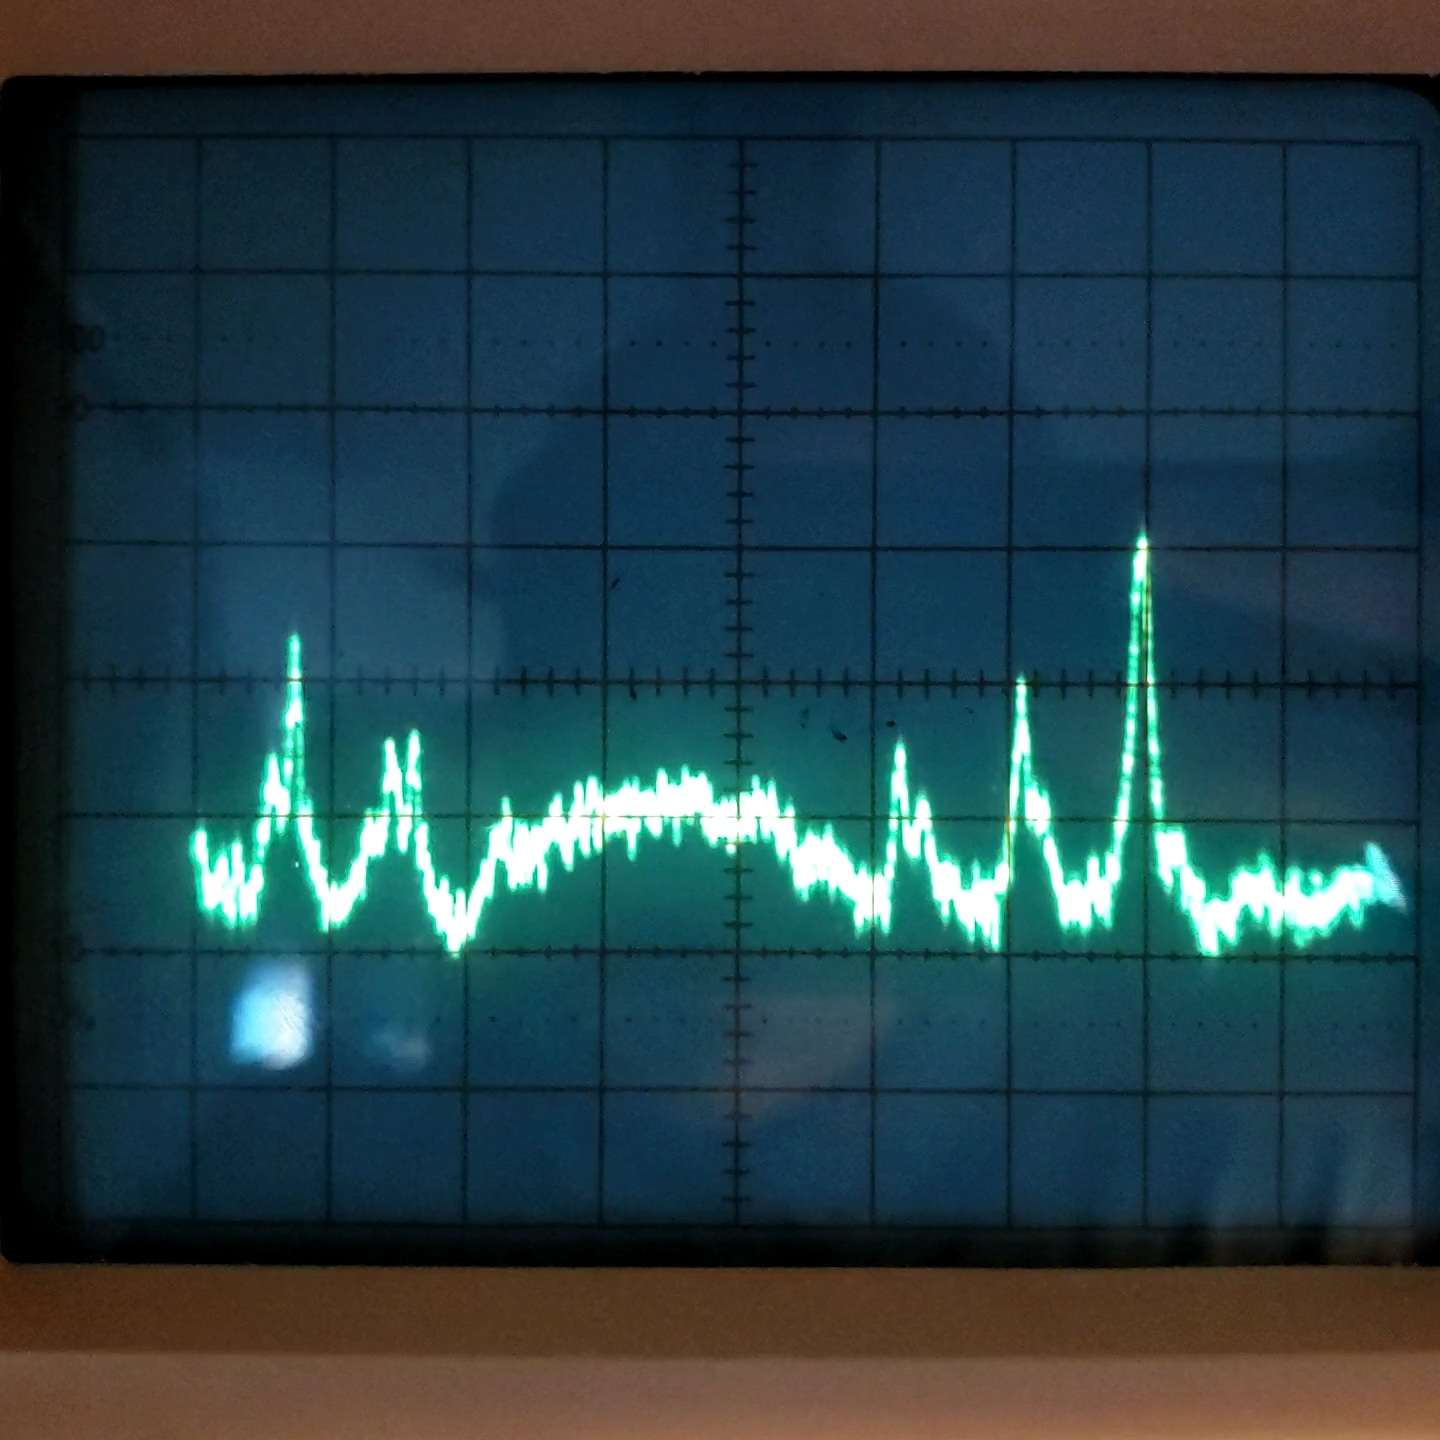
\includegraphics[width=\textwidth]{oscLow.jpg}
         \caption{}
         \label{fig:low}
     \end{subfigure}
        \caption{Изменение изображения при уменьшении напряжения от максимального \ref{fig:high} до минимального \ref{fig:low}}
        \label{fig:oscs}
\end{figure}

\subsection{Измерения}
Так как единственное значение, не являющееся табличным в данной работе~--- количество мод, укладывающихся в ширину контура, погрешность определения коего затруднительно оценить, то дальнейшие результаты являются качественными, а погрешность их определения не оценивается.

Параметры установки: $L = 65\text{ см}$~--- длина резонатора лазера, $l = 9\text{ см}$~--- длина резонатора интерферометра, $\lambda = 6328 \si{ \angstrom}$~--- длина волны лазера, $f = \nu = \frac {c}{\lambda} = 473,8 \cdot 10^{12} \text{ Гц}$~--- его частота, $\nu_V = 50 \text{ Гц}$~--- частота работы пьезоэлектрического элемента.

На основании приведенных выше данных и формулы \eqref{modeDiff} получим межмодовое расстояние лазера: 
\[
\delta \nu = \nu_{m + 1} - \nu_{m} = \frac {c}{2L} = \frac {3 \cdot 10^{10} \text{см/с}}{2 \cdot 65 \text{ см}} = 2,3 \cdot 10^8 \text{ Гц}.
\]
\begin{figure}[hb]
    \centering
    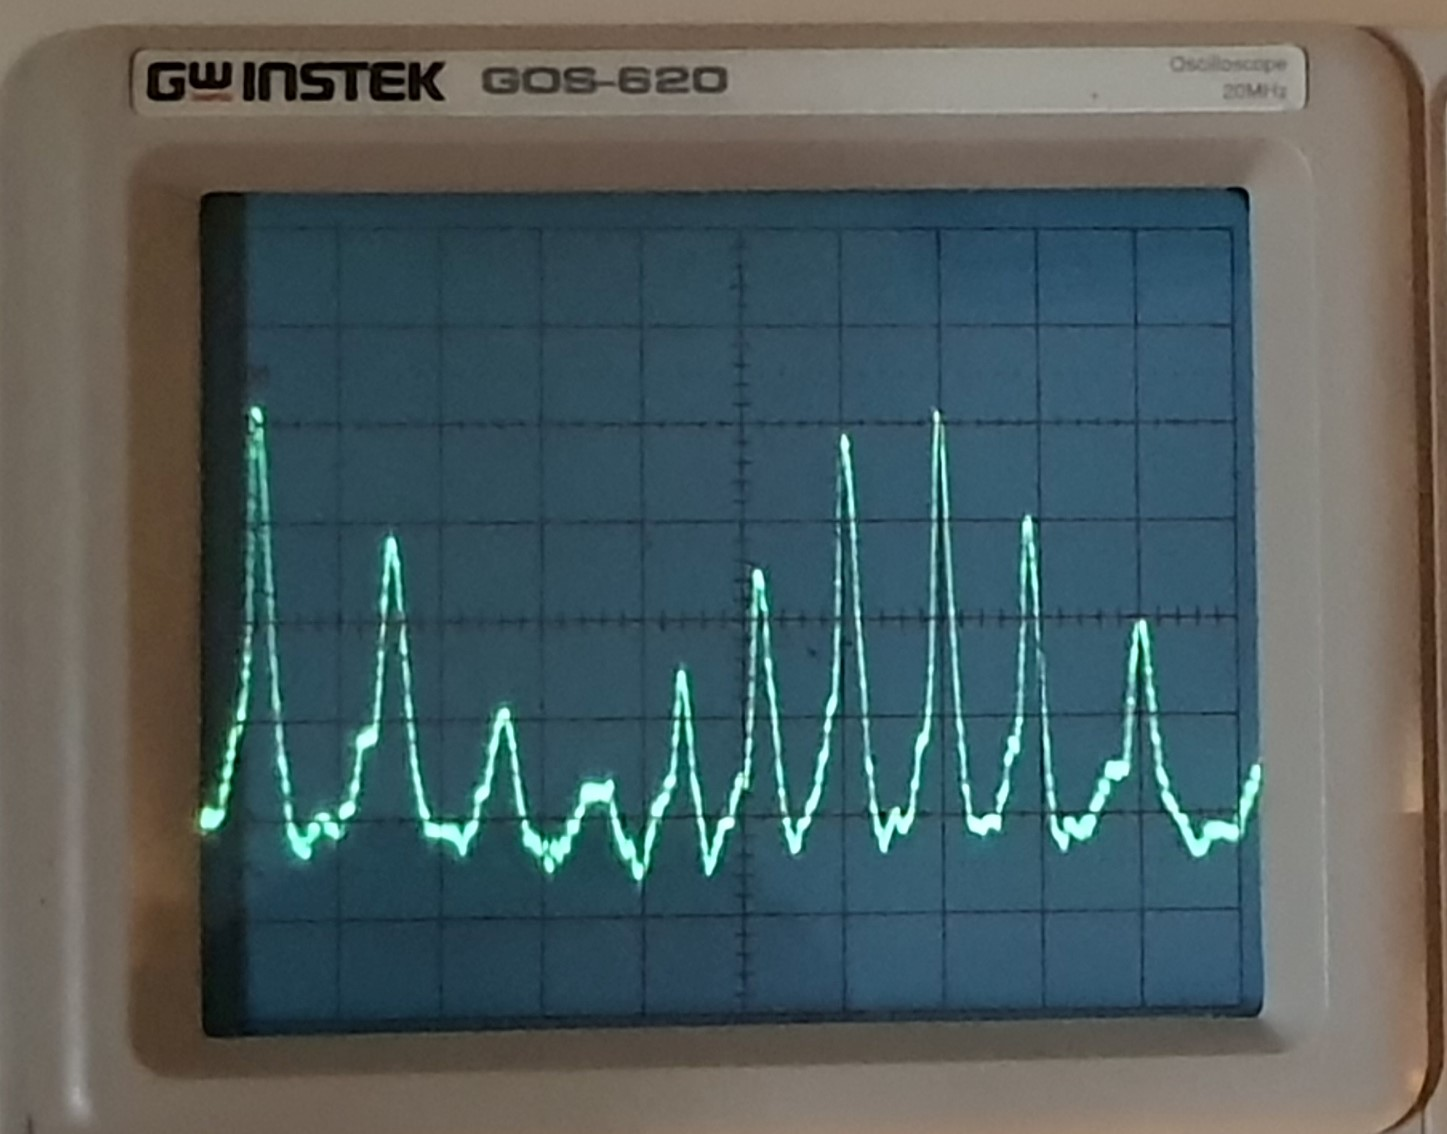
\includegraphics[width=0.6\textwidth]{oscar_3.jpg}
    \caption{Осциллограмма спектра лазерного излучения, число пиков в доплеровском контуре}
    \label{fig:oscar_3}
\end{figure}
В ходе эксперимента на экране осциоллографа наблюдалось, что в однин доплеровский контур укладывается $n = 8$ пиков~--- мод, генерируемых лазером (см. рис. \ref{fig:oscar_3}). Это соответствует ширине доплеровского контура в $7$ межмодовых расстояний, то есть 
\[
\Delta \nu(\text{Ne}) = n \cdot \delta \nu = 7 \cdot 2,3 \cdot 10^8 \text{ Гц} = 1,6 \text{ ГГц}.
\]
Используя следствия закона Доплера \eqref{dope}, оценим среднюю скорость атомов неона:
\[
\frac{\Delta \lambda_D}{\lambda} = 
\frac{\Delta \nu (\text{Ne}) }{ \nu } \approx 
\frac{v_x}{c} \Longrightarrow 
v_x \approx c \frac{\Delta \nu (\text{Ne})}{\nu} = 
\frac{1,6 \cdot 10^9}{473,8 \cdot 10^{12}} \cdot 3 \cdot 10^{10} \text{ см/с} \approx 1,01 \cdot 10^5 \text{ см/с}.
\]
Пользуясь соотношением \eqref{cool_DoppWidth}, оценим газокинетическую температуру разряда:
\begin{gather*}
\Delta\nu_D = \sqrt{\ln 2}\cdot\frac{\nu_{max}}{c}\sqrt{\frac{2kT}{m}} \Longrightarrow 
T = \left(\frac{c\cdot \Delta \nu_D }{\nu_{max} \sqrt{\ln{2}}} \right)^2 \frac{m}{2k} \\
T = \left(\frac{3 \cdot 10^8 \cdot 1,6 \cdot 10^9 }{473,8 \cdot 10^{12}} \right)^2 \cdot \frac{20,2 \cdot 1,66 \cdot 10^{-27}}{2 \cdot 1,38 \cdot 10^-23 \cdot \ln(2)} \approx 1800 \text{ К}.
\end{gather*}

\subsection{Разрешающая способность интерферометра}
Далее рассчитаем дисперсионную область сканирующего интерферометра, пользуясь соотношением, аналогичным соотношению \eqref{modeDiff}:
\[
\Delta \lambda_{\text{си}} = \frac {\lambda} {m} = \frac {\lambda ^2}{2l} = \frac{(6328 \cdot 10^{-8} \text{ см})^2}{2 \cdot 9 \text{ см}} \approx 2.2 \cdot 10^{-10} \text{ см} = 0,022 \si{\angstrom}.
\]
Сравним с видимой шириной линии неона: 
\[
\Delta \lambda (\text{Ne}) = \Delta \nu (\text{Ne}) \cdot \frac {\lambda^2}{c} =
1,6 \cdot 10^9 \cdot \frac{(6328 \cdot 10^{-8})^2}{3 \cdot 10^{10}} = 2,1 \cdot 10^{-10} \text{ см} = 0,0021 \si{\angstrom}.
\]
Тот факт, что дисперсионная область интерферометра близка к ширине контура означает, что длина интерферометра подобрана оптимально для данного излучения, и интерферометр способен обеспечить максимальную разрешающую способность.

Измерив отношение ширины отдельной моды на полувысоте к межмодовому расстоянию, можно получить разрешение $\delta \lambda$ сканирующего интерферометра и разрешающую способность:
\[
\delta \lambda = \frac{\lambda^2}{2 L} \cdot \frac{1,1}{10} = 0,00308 \cdot \frac{1,1}{10} \si{\angstrom} = 3,39 \cdot 10^{-12}\text{ см} = 0,000339 \si{\angstrom}.
\]
Разрешающую способность найдем, воспользовавшись соотношением \eqref{eq:R}:
\[
R = \frac{\lambda}{\delta \lambda} = \frac{6328}{0,000339} \approx 1,86 \cdot 10^7.
\]
Пользуясь формулой \eqref{eq:R_r}, оценим коэффициент отражения зеркал:
\[
r = 1 - \frac{2 \pi l} {\lambda R} = 
1 - \frac{2 \pi \cdot 9 \text{см}} {6328 \cdot 10^{-8} \text{см} \cdot 1,68 \cdot 10^7 } \approx 0,95.
\]
Полученное значение довольно близко к представленному в описании работы (около 98,5\%).
\newpage

\section{Выводы}
В ходе работы удалось оценить качественные и количественные характиеристики лазерного излучения гелий-неонового лазера, а также исследовать его модовый состав. 
\begin{itemize}
    \item Эффект Доплера заметно наблюдается на спектральной картине излучения.
    \item Лазер работает в режиме многомодовой генерации.
    \item Средняя скорость движения атомов, рассчитанная на основе закона Доплера, составляет $v_x \approx 1,01 \cdot 10^5 \text{см/с}$, что вполне соответствует по порядку скорости свободного пробега атомов в разреженном газе.
    \item Газокинетическая температура разряда оценивается в $T = 1800K$, что хорошо сходится с приблизительными значениями для установок данного типа. Последние два результата позволяют утверждать, что ширину спектра лазера действительно можно считать определяемой преимущественно эффектом Доплера.
\end{itemize}
Также в работе исследован сканирующий интерферометр. 
\begin{itemize}
    \item При уменьшении амплитуды напряжения на пьезоэлементе число мод, укладывающихся на спектральной картине уменьшается. Также слегка меняется ее вид, что обусловлено изменением амплитуды колебаний по отношению к длине волны лазера.
    \item Дисперсионная область интерферометра сравнима с шириной доплеровского контура, из чего следует высокая точность и разрешающая способность прибора. 
    \item Рассчитанное разрешение интерферометра составляет $\delta \lambda = 0,0021 \si{\angstrom}$, что приводит к значению разрешающей способности порядка $R = 1,86 \cdot 10^7$. 
    \item На основании теоретической формулы для разрешающей способности сканирующего интерферометра Фабри-Перо коэффициент отражения зеркал получен $r \approx 95\%$, что неплохо сходится с табличными значениями для установок данного типа (около $95\%$).
\end{itemize}